% Primarily this section should be about scientific methods and theories you need to evaluate/compare/invent to solve your problems from 1.3.
% In some cases it may be ok to describe different technologies, but the purpose is to describe something and then draw a conclusion from that.
% Example, if you decide to discuss different databases, it may be for the purpose of selecting the best type for your implementation later on (based on for example data representation, scalability, speed, etc.).
% Optimally the problems in 1.3 are not solved by anyone else yet, in which case this section needs to describe how to solve them (new algorithms, mathematical approaches, etc.).
 
% This section can have a lot of subsections (3.1, 3.2, 3.3, etc).

% TODO: Explain DWARF Die

One of the most important data structures in the \gls{DWARF} format is the \gls{die}.
A \gls{die} is low level representation of a small part of the source code.
Some of the most common things \glspl{die} represent are functions, variables and types.
The \glspl{die} are found in a tree structure referred to as a \gls{die} tree.
Each \gls{die} tree will often represent a whole compile unit or a type from the source code.
The ones representing compile units are found in the \gls{DWARF} section \emph{.debug\_info}, while the ones representing type are found in the \gls{DWARF} section \emph{.debug\_type}.
The \glspl{die} representing types are often referred to as type \glspl{die}.


%The information stored in \glspl{die} are all in the form of \gls{DWARF} attributes.
%There are a lot of different attributes a \gls{die} can have, but they never have more then one of the same.
%The information in the attributes varies a lot depending on what attribute it is.


% TODO: Explain DWARF Attributes
\subsubsubsection{Dwarf Attribute}
\subimport{}{dwarf-attribute.tex}


\subsubsubsection{Example of a DIE}%\gls{die}}
Looking at an example of a \gls{die} that describes a variable.
The example can be seen in figure \ref{fig:dwarfdie} which is a screenshot of the output from the program \emph{objdump} run on a \gls{elf} file.
The first line in the figure begins with a number $8$ which represents the depth in the \gls{die} tree this \gls{die} is located.
The next number is the current lines offset into this compile unit, all the other lines in the figure also start with their offset.
Then it says "Abbrev Number: 9" on the same line, this is an abbreviation code that translates to \emph{DW\_TAG\_variable}.
This tag means that the \gls{die} is representing a variable from the source code.


\begin{figure}[h]
	\centering
	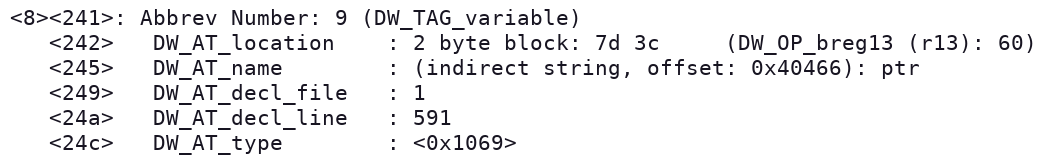
\includegraphics[width=1.0\textwidth]{dwarf-die.png}
	\caption{An example of a \gls{die} representing a variable named \emph{ptr}. This example is the output of the tool \emph{objdump} run on a \gls{DWARF} file.}
	\label{fig:dwarfdie}
\end{figure}


The attribute \emph{DW\_AT\_location} seen in figure \ref{fig:dwarfdie} has the information of where the variable is stored on the debug target.
The attribute \emph{DW\_AT\_name} has an offset into the \gls{DWARF} section \emph{.debug\_str} that the \emph{objdump} tool has evaluated to "str", this is the name of the variable.
Attributes \emph{DW\_AT\_decl\_file} and \emph{DW\_AT\_decl\_line} in the figure contain  offsets into the section \emph{.debug\_line}.
Those offsets can be evaluated to the source file path and line number that this \gls{die} is generated from.
Lastly the attribute \emph{DW\_AT\_type} contain an offset into the section \emph{.debug\_types}, that points to a type \gls{die} that has the type information for this variable.


